\apendice{Documentación técnica de programación}

\section{Introducción}


\section{Estructura de directorios}

\section{Manual del programador}


\subsection{Instalación y configuración de GWT:}


Para poder trabajar con GWT \footnote{\url{http://www.oracle.com/technetwork/java/javase/downloads/index.html}}, se debe descargar el SDK de GWT proporcionado en la página web oficial. Los requisitos previos para crear un aplicación web con Google Web Toolkit son básicamente dos: tener instalada la SDK de Java en su versión 1.6 o cualquiera superior a esta y tener instalado también Apache Ant o en su defecto Apache Maven.

Es fácil saber si cumplo ambos requisitos. Una vez descargado el SDK de GWT desde la página oficial, accedo a la carpeta desde la consola de comandos, y ahí intento ejecutar el comando <<webAppCreator>>. En caso de que la consola me devuelva un error en el que indica que Java no ha podido reconocerlo como un comando interno, quiere decir que no cumplo esos requisitos previos.

Posteriormente puedo proceder de varias formas y con diferentes plataformas.
En mi caso he elegido la plataforma Eclipse sobre la que trabajaré en su
versión 4.4 que es también denominada  con el nombre de Luna.

GWT se instala en Eclipse como un <<plugin>> y para ello debo ir, dentro de Eclipse a <<añadir un nuevo software>> donde encontraremos una ventana donde escribir la dirección del software a instalar. Para mi versión la URL es \footnote{\url{https://developers.google.com/eclipse/docs/install-eclipse-4.4}} que una vez añadida mostrará los paquetes a instalar. Estos deben ser Google Plugin for Eclipse y GWT Designed for GPE, y una vez seleccionados se procederá a su instalación normal. Después de reiniciar procedo a referenciar el SDK de GWT yendo a <<preferencias>>, <<Google>> y dentro de <<Web Toolkit>> añadir el SDK que descargué anteriormente. 

Para añadir un nuevo proyecto a Eclipse tengo que importarlo desde Maven, puedo hacerlo añadiendo un proyecto de Maven existente. Una vez seleccionado el proyecto, hay que configurar su ejecución. Debemos ir a <<Run Configuration>> y seleccionar el constructor de Maven. Una vez ahí, puedo añadirle un nombre específico y seleccionando el directorio base el proyecto a ejecutar y por último el <<Goal>>, o meta debe ser <<gwt:run>>, ya que en caso contrario no se producirá una ejecución correcta.

Antes de la ejecución se debe instalar el constructor de Maven desde el debuguer, sino puede dar algunos errores. Una vez finalizada la instalación, podremos ejecutar un proyecto con GWT apareciendo así el modo desarrollador y ahí se podrá lanzar la aplicación en el buscador por defecto.

El <<plugin>> de GWT es sencillo de utilizar y solo con hacer click en <<New Web Application Project>> aparecerá un <<wizard>> en el cual hay que introducir el nombre del proyecto y el paquete principal. Se recomienda desmarcar <<Use Google App Engine>> ya que además de que no nos interesa, puede que nos dé algún error. Hecho esto se creará un proyecto automáticamente en forma de ejemplo, con un paquete cliente, otro servidor y uno compartido.


(05/03/2017)
Los proyectos en GWT se componen de una parte cliente y otra servidor. He creado un proyecto con sólo la parte del cliente, la cual es la más importante. En el paquete <<src/client>> he incluido la clase principal que llamará a las otras. En realidad no se si esto es correcto al cien por cien.
Solución del error del  <<prefuse>> es descargando de la página oficial \footnote{\url{http://prefuse.org/}} el proyecto, incluyo el paquete prefuse y añado, desde <<Java Build Path>> la librería  <<lucene>> porque es necesaria para algunas clases del paquete. Inicialmente muestra unos errores del tipo <<did you forget to inherit a required module?>> referente a que dentro del proyecto, la clase con extensión .gwt.xml no incluye algunas de las rutas de los recursos que utilizo. No estiendo muy bien el error. (continuar con la explicación)


 
\subsection{Parser JavaCC}

GWT esta compuesto por una parte cliente, que es la que será traducida a JavaScript, y otra servidor escrita en Java y que no se traducirá. En un principio se prueba a incluir toda la aplicación dentro del lado del cliente, traduciendo todo a JavaScript. Pero como ya se ha dicho en otros apartados, GWT sólo soporta unas determinadas librerías en dicho lado y tiene algunas restricciones más\footnote{Para más detalles visite\url{http://www.gwtproject.org/doc/latest/DevGuideCodingBasicsCompatibility.html}.} que obligan a incluir el parser de JavaCC en el servidor, en vez del cliente.

Originalmente en el núcleo de Thoth dentro del directorio <<grammar>> colgaba un sub-directorio llamado <<parserjavacc>> en el cual se encontraba el parser para la gramática. Es la parte más importante dentro de la gramática ya que permite reconocer si esta está bien construida o no.
Ahora no procede explicar que es, pero si en que ha cambiado esta versión con respecto a la anterior. 
Para poder incluir esa parte en el proyecto decidimos hacerlo en el lado del servidor, ya que al no hacerse la traducción no habría ningún problema. Ahora bien lo más complicado de todo esto es la comunicación entre esas dos partes.



\subsection{Comunicación cliente-servidor}
Una vez alojado en el servidor el parser habrá que establecer una comunicación entre la parte del ciente en la que habrá un método que llame a la funcionalidad que se desee del servidor.

Para hacerlo, GWT utiliza la técnica denominada por sus siglas en inglés RPC o llamada de procedimiento remoto (Remote Procedure Call) que tiene una estructura similar a la siguiente ilustración \ref{fig:5.1}.

\begin{figure}[h]
\centering
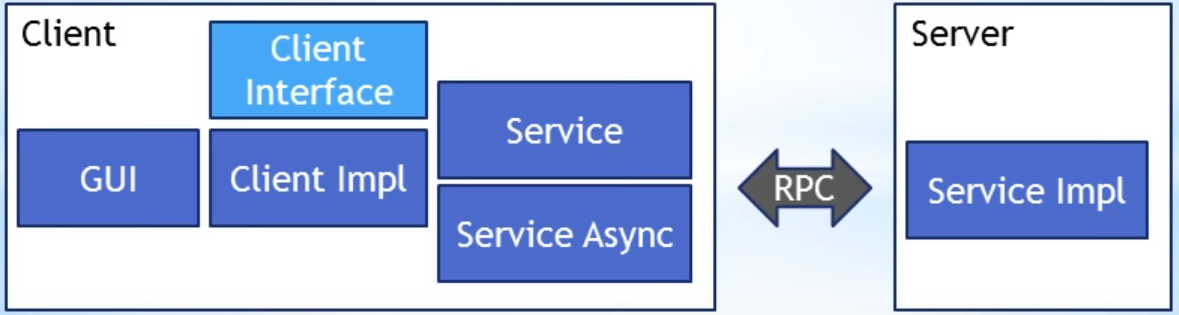
\includegraphics[width=0.65\textwidth]{RPC}
\caption{Arquitectura RPC simple. Fuente propia.}
\label{fig:5.1}
\end{figure}

Del lado del cliente tenemos, en este caso, una interfaz gráfica de usuario (GUI), una clase dedicada a hacer las llamadas RPC (ClienImpl), dos interfaces que definen los métodos (Service y ServiceAsync), una clase con los métodos en el lado del servidor (serviceImpl) y por último una interfaz, que no es esencialmente necesaria (ClientInterface). 

En términos generales, para utilizar el parser de la gramática, que es quizá la clave de todo, hay que llamar al servidor y establecer una comunicación. Es ahí donde utilizamos la clase <<GrmmarServiceClientImp>> que hace las llamadas a las interfaces necesarias hasta llegar al servidor. Esta clase es un nexo de unión entre la parte del núcleo, que ese encuentra en el servidor, y la parte del cliente, que contiene lo visual y las acciones de los botones entre otros. La comunicación queda representada en este diagrama\ref{fig:5.2}.

\begin{figure}[h]
\centering
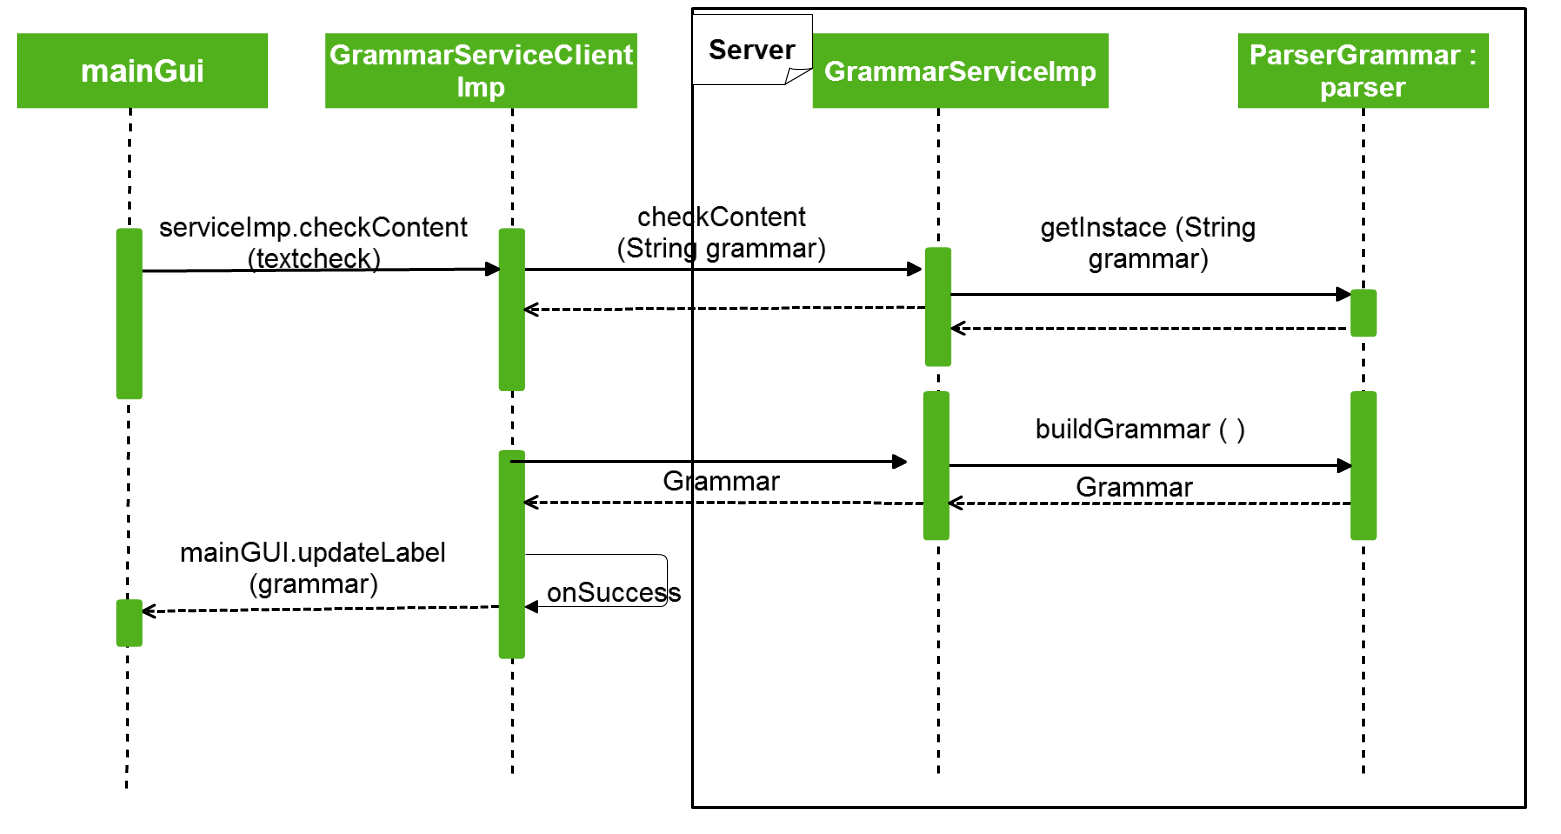
\includegraphics[width=1.1\textwidth]{ParserDiagram}
\caption{Diagrama sobre la comunicación entre el cliente y el servidor en GWT.}
\label{fig:5.2}
\end{figure}

Dentro de la clase <<GrammarServiceClientImp>> hay tres constructores según le pasemos una gramática, un texto, simplemente nada. El atributo url es simplemente la localización del <<servlet>> que se utiliza para la comunicación RPC. Estos detalles se aprecian mejor en el diagrama de clases que muestra la siguiente imagen \ref{fig:5.3}.

\begin{figure}
\raggedleft
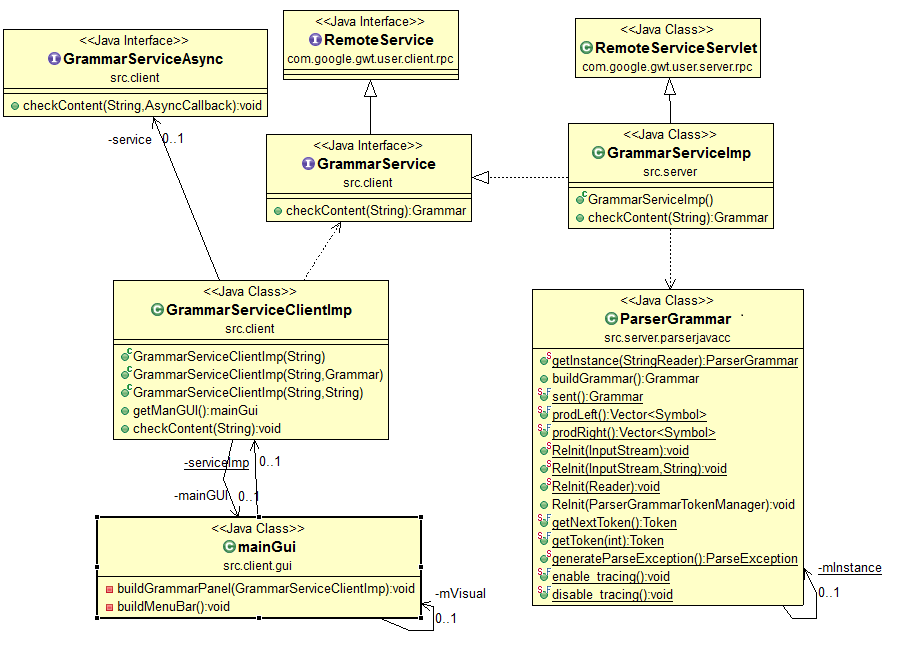
\includegraphics[scale=0.9]{Parser-ClassDiagram}
\caption{Diagrama de clases que muestra como utiliza el parser de la gramática. Diagrama realizado con ObjectAid.}
\label{fig:5.3}
\end{figure}

\section{Compilación, instalación y ejecución del proyecto}

\section{Pruebas del sistema}
